\documentclass[a4paper,UKenglish,cleveref, autoref, thm-restate]{lipics-v2021}
%This is a template for producing LIPIcs articles. 
%See lipics-v2021-authors-guidelines.pdf for further information.
%for A4 paper format use option "a4paper", for US-letter use option "letterpaper"
%for british hyphenation rules use option "UKenglish", for american hyphenation rules use option "USenglish"
%for section-numbered lemmas etc., use "numberwithinsect"
%for enabling cleveref support, use "cleveref"
%for enabling autoref support, use "autoref"
%for anonymousing the authors (e.g. for double-blind review), add "anonymous"
%for enabling thm-restate support, use "thm-restate"
%for enabling a two-column layout for the author/affilation part (only applicable for > 6 authors), use "authorcolumns"
%for producing a PDF according the PDF/A standard, add "pdfa"

%\pdfoutput=1 %uncomment to ensure pdflatex processing (mandatatory e.g. to submit to arXiv)
\hideLIPIcs  %uncomment to remove references to LIPIcs series (logo, DOI, ...), e.g. when preparing a pre-final version to be uploaded to arXiv or another public repository

%\graphicspath{{./graphics/}}%helpful if your graphic files are in another directory

\bibliographystyle{plainurl}% the mandatory bibstyle

\title{\textsf{weberknecht}}

%\titlerunning{Dummy short title} %TODO optional, please use if title is longer than one line

\author{Johannes Rauch}
{Ulm University, Institute of Optimization and Operations Research, Germany}
{johannes.rauch@uni-ulm.de}
{https://orcid.org/0000-0002-6925-8830}
{}%TODO mandatory, please use full name; only 1 author per \author macro; first two parameters are mandatory, other parameters can be empty. Please provide at least the name of the affiliation and the country. The full address is optional. Use additional curly braces to indicate the correct name splitting when the last name consists of multiple name parts.

\authorrunning{J. Rauch} %TODO mandatory. First: Use abbreviated first/middle names. Second (only in severe cases): Use first author plus 'et al.'

\Copyright{Johannes Rauch} %TODO mandatory, please use full first names. LIPIcs license is "CC-BY";  http://creativecommons.org/licenses/by/3.0/

\ccsdesc[500]{Mathematics of computing~Graph algorithms}
%TODO mandatory: Please choose ACM 2012 classifications from https://dl.acm.org/ccs/ccs_flat.cfm 

\keywords{One-Sided Crossing Minimization}%TODO mandatory; please add comma-separated list of keywords

%\category{} %optional, e.g. invited paper

%\relatedversion{} %optional, e.g. full version hosted on arXiv, HAL, or other respository/website
%\relatedversiondetails[linktext={opt. text shown instead of the URL}, cite=DBLP:books/mk/GrayR93]{Classification (e.g. Full Version, Extended Version, Previous Version}{URL to related version} %linktext and cite are optional

\supplement{!!!!!!!!!!!!!!}%optional, e.g. related research data, source code, ... hosted on a repository like zenodo, figshare, GitHub, ...
%\supplementdetails[linktext={opt. text shown instead of the URL}, cite=DBLP:books/mk/GrayR93, subcategory={Description, Subcategory}, swhid={Software Heritage Identifier}]{General Classification (e.g. Software, Dataset, Model, ...)}{URL to related version} %linktext, cite, and subcategory are optional

%\funding{(Optional) general funding statement \dots}%optional, to capture a funding statement, which applies to all authors. Please enter author specific funding statements as fifth argument of the \author macro.

\acknowledgements{I thank Henning Bruhn-Fujimoto and Dieter Rautenbach for helpful discussions.}%optional

%\nolinenumbers %uncomment to disable line numbering



%Editor-only macros:: begin (do not touch as author)%%%%%%%%%%%%%%%%%%%%%%%%%%%%%%%%%%
\EventEditors{Philipp Kindermann and Fabian Klute and Soeren Terziadis}
\EventNoEds{3}
\EventLongTitle{Parameterized Algorithms and Computational Experiments 2024}
\EventShortTitle{PACE 2024}
\EventAcronym{PACE}
\EventYear{2024}
\EventDate{2023--2024}
\EventLocation{}
\EventLogo{}
\SeriesVolume{$\times$}
\ArticleNo{$\times$}
%%%%%%%%%%%%%%%%%%%%%%%%%%%%%%%%%%%%%%%%%%%%%%%%%%%%%%

\usepackage{tikz}
\tikzset{
	dot/.style = {circle, fill, minimum size=#1,
		inner sep=0pt, outer sep=0pt},
	dot/.default = 5pt
}

\newcommand{\OSCM}{\textsc{One-Sided Crossing Minimization}}

\begin{document}

\maketitle

%TODO mandatory: add short abstract of the document
\begin{abstract}
This article describes the implementation of \textsf{weberknecht(\_h)}\footnote{Weberknecht is the german name for the harvestman spider. It is a composite word consisting of the words Weber = weaver and Knecht = workman. 
%One may find a similarity between the bipartite input graphs and a textile mounted to a loom, which inspired the name.
}, a solver for \OSCM{} that participated in the Parameterized Algorithms and Computational Experiments Challenge 2024.
\end{abstract}

\section{Preliminaries}\label{sec:pre}
An instance $(G = (A, B, E), \pi_A)$ of \OSCM{} is a bipartite graph $G$ with $n$ vertices, bipartition sets $A$ and $B$, and a linear ordering $\pi_A$ of $A$.
The goal is to find a linear ordering $\pi_B$ of $B$ that minimizes the number of crossing edges if the graph were to be drawn in the plane such that
\begin{itemize}
	\item the vertices of $A$ and $B$ are on two distinct parallel lines, respectively, and 
	\item the order of the vertices of $A$ and $B$ on the lines is consistent with $\pi_A$ and $\pi_B$, respectively.
\end{itemize}
We assume that $A = [n_0] := \{1, \dots, n_0\}$ and $B = \{n_0 + 1, \dots, n_0 + n_1\}$ for some positive integers $n_0$ and $n_1$.
We think of $\pi_A$ and $\pi_B$ as bijections $A \rightarrow [n_0]$ and $B \rightarrow [n_1]$, respectively.
If $\pi_B(u) < \pi_B(v)$ for $u, v \in B$, we say that $u$ is ordered before $v$, or $u$ is to the left of $v$.

Let $c_{u,v}$ denote the number of crossings of edges incident to $u, v \in B$ if $\pi_B(u) < \pi_B(v)$.
A mixed-integer program for \OSCM{} is given by
\begin{equation}
\label{mip}
\begin{alignedat}{2}
\text{minimize } &\sum_{\substack{u, v \in B\\u < v}} (c_{u,v} - c_{v,u}) \cdot x_{u,v} + \sum_{\substack{u, v \in B\\u < v}} c_{v,u}\\
\text{subject to } &\begin{aligned}[t]
0 \leq x_{u,v} + x_{v,w} - x_{u,w} \leq 1 &\quad\text{for all }u,v,w \in B, u < v < w,\\
x_{u,v} \in \{0,1\} &\quad\text{for all }u,v \in B, u < v.
\end{aligned}
\end{alignedat}\tag{$P_I$}
\end{equation}
So, $u$ is ordered before $v$ if and only if $x_{u,v} = 1$ for $u, v \in B, u < v$.

%, with smaller values of $\pi_A$ and $\pi_B$ meaning ``more left''.
%See the handbook , Chapter 13, for an introduction to the topic.
%Note that the total number of crossings depends only on the relative positions of all unordered pairs of vertices.

\section{Overview}
The solver \textsf{weberknecht(\_h)} is written in C++.
First, the exact solver \textsf{weberknecht} runs the uninformed and improvement heuristics described in Section~\ref{sec:heu}.
Then it applies the data reduction rules described in Section~\ref{sec:red}.
Last, it solves a reduced version of the mixed-integer program associated to the input instance with a custom branch and bound and cut algorithm described in Section~\ref{sec:bnb}.
The heuristic solver \textsf{weberknecht\_h} only runs the uninformed and improvement heuristic (except the local search heuristic).


\section{Heuristics}\label{sec:heu}
We distinguish between uninformed and informed heuristics, which build a solution from the ground up, and improvement heuristics, which try to improve a given solution.
Due to the reduction rules we may assume from here that there are no isolated vertices in $G$.

\medskip
\noindent
\textbf{Uninformed Heuristics.}
The uninformed heuristics order the vertices of $B$ such that the \emph{scores} $s(v)$ of vertices $v \in B$ is non-decreasing:
\begin{itemize}
\item In the \emph{barycenter heuristic}, we have $s(v) = \frac{1}{d_G(v)} = \sum_{u \in N_G(v)} u$ (recall that $A = [n_0]$). Eades and Wormald~\cite{eades1994edge} proved that this method has an $\mathcal{O}(\sqrt{n})$ approximation factor, which is best possible up to a constant factor under certain assumptions.
\item Let $d = d_G(v)$ and let $\{w_0, \dots, w_{d-1}\}$ be the neighbors of $v$ in $G$ with $w_0 < \dots < w_{d-1}$.
In the \emph{median heuristic}, the score of $v$ is $s(v) = w_{(d-1)/2}$ if $d$ is odd and $s(v) = (w_{d/2 - 1} + w_{d/2})/2$ if $d$ is even.
Eades and Wormald~\cite{eades1994edge} proved that this method is a factor three approximation algorithm.
\item In the \emph{probabilistic median heuristic}, we draw a value $x$ from $[0.0957, 0.9043]$ uniformly at random, and the score of $v$ is then $s(v) = w_{\lfloor x \cdot d \rfloor}$.
This is essentially the approximation algorithm of Nagamochi~\cite{nagamochi2005improved}, which has an approximation factor of $1.4664$ in expectancy.
\end{itemize}

\noindent
\textbf{Informed Heuristics.}
The informed heuristics get a fractional solution of the linear program relaxation of \eqref{mip} as an additional input.
\begin{itemize}
\item The \emph{sort heuristic} works like the uninformed heuristics.
The score for vertex $v \in B$ is $s(v) = \sum_{u \in B, u < v} x_{u,v} + \sum_{u \in B, v < u} (1 - x_{v, u})$.
\item Classical \emph{randomized rounding heuristic}.
\item \emph{Relaxation induced neighborhood search}~\cite{danna2005exploring}.
\end{itemize}

\noindent
\textbf{Improvement Heuristics.}
Assume that $\pi_B = u_1u_2 \dots u_{n_1}$ is the current best solution.
\begin{itemize}
\item The \emph{shift heuristic} that Grötschel et al.~\cite{grotschel1984cutting} describes tries if shifting a single vertex improves the current solution.
\item In the \emph{local search heuristic}, we solve a reduced version of \eqref{mip} to optimality, where we only add variables $x_{u_i, u_j}$ with $|i-j| < w$ for some parameter $w$.
\end{itemize}

\section{Data Reduction}\label{sec:red}
The solver \textsf{weberknecht} implements the following data reduction rules:
\begin{itemize}
\item Vertices of degree zero in $B$ are put on the leftmost positions in the linear ordering $\pi_B$.
\item Let $l_v$ ($r_v$) be the neighbor of $v \in B$ in $G$ that minimizes (maximizes) $\pi_A$, respectively.
Dujmovi\'c and Whitesides~\cite{dujmovic2004efficient} noted that, if there exists two nonempty sets $B_1, B_2 \subseteq B$ and a vertex $q \in A$ such that for all $v \in B_1$ we have that $\pi_A(r_v) \leq \pi_A(q)$, and for all $v \in B_2$ we have that $\pi_A(q) \leq \pi_A(l_v)$,
then the vertices of $B_1$ appear before the vertices $B_2$ in an optimal solution.
In this case we can split the instance into two subinstances.
%$$(G_i = (A_i = N_G(B_i), B_i, E[A_i \cup B_i]), \pi_A|_{A_i}) \quad \text{for $i=1,2$}.$$
\item Dujmovi\'c and Whitesides~\cite{dujmovic2004efficient} proved that, 
if $\pi_B$ is an optimal solution, and $c_{u, v} = 0$ and $c_{v, u} > 0$,
then $\pi_B(u) < \pi_B(v)$.
\item Dujmovi\'{c} et al.~\cite{dujmovic2008fixed} described a particular case of the next reduction rule.
Let $c_{u, v} < c_{v, u}$. 
We describe the idea with the example in Figure~\ref{fig:rr}.
Imagine that we draw some edge $x_iy_j$ into Figure~\ref{fig:rr}.
If the number of edges crossed by $x_iy_j$ on the left side is at most the number of edges crossed by $x_iy_j$ on the right side for all edges of the form $x_iy_j$, then we have $\pi_B(u) < \pi_B(v)$ in any optimal solution $\pi_B$:
Otherwise we could improve the solution by simply exchanging the positions of $u$ and $v$.
Note that this reduction rule is only applicable if $d_G(u) = d_G(v)$ as witnessed by $x_2y_1$ and $x_2y_k$ ($k=5$ here).
\item The value $\ell b = \sum_{u, v \in B, u < v} \min(c_{u,v}, c_{v,u})$ is a lower bound on the number of crossings of an optimal solution.
Suppose that we have already computed a solution with $ub$ crossings.
Then, if $c_{u,v} \geq ub - \ell b$ for some $u, v \in B$, it suffices to only consider orderings $\pi_B$ with $\pi_B(u) > \pi_B(v)$ for the remaining execution.
\item After the execution of the described reduction rules, some variables $x_{u,v}$ of $(P_I)$ have a fixed value due to the constraints.
\end{itemize}

\begin{figure}
\centering
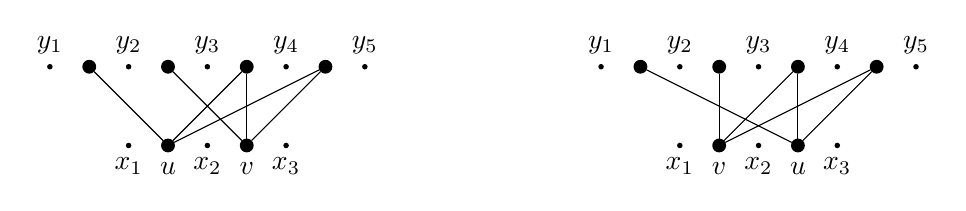
\begin{tikzpicture}
\begin{scope}[xscale=0.5, shift={(-7,0)}]
\node[dot=2, label=below:$x_1$] (x1) at (-2,0) {};
\node[dot, label=below:$u$] (u) at (-1,0) {};
\node[dot=2, label=below:$x_2$] (x2) at (0,0) {};
\node[dot, label=below:$v$] (v) at (1,0) {};
\node[dot=2, label=below:$x_3$] (x3) at (2,0){};

\node[dot=2, label=above:$y_1$] at (-4,1) {};
\node[dot] (n1) at (-3,1) {};
\node[dot=2, label=above:$y_2$] at (-2,1) {};
\node[dot] (n2) at (-1,1) {};
\node[dot=2, label=above:$y_3$] at (0,1) {};
\node[dot] (n3) at (1,1) {};
\node[dot=2, label=above:$y_4$] at (2,1) {};
\node[dot] (n4) at (3,1) {};
\node[dot=2, label=above:$y_5$] at (4,1) {};

\draw (n1) to (u);
\draw (n3) to (u);
\draw (n4) to (u);
\draw (n2) to (v);
\draw (n3) to (v);
\draw (n4) to (v);
\end{scope}
\begin{scope}[xscale=0.5, shift={(7,0)}]
\node[dot=2, label=below:$x_1$] (x1) at (-2,0) {};
\node[dot, label=below:$u$] (u) at (1,0) {};
\node[dot=2, label=below:$x_2$] (x2) at (0,0) {};
\node[dot, label=below:$v$] (v) at (-1,0) {};
\node[dot=2, label=below:$x_3$] (x3) at (2,0){};

\node[dot=2, label=above:$y_1$] at (-4,1) {};
\node[dot] (n1) at (-3,1) {};
\node[dot=2, label=above:$y_2$] at (-2,1) {};
\node[dot] (n2) at (-1,1) {};
\node[dot=2, label=above:$y_3$] at (0,1) {};
\node[dot] (n3) at (1,1) {};
\node[dot=2, label=above:$y_4$] at (2,1) {};
\node[dot] (n4) at (3,1) {};
\node[dot=2, label=above:$y_5$] at (4,1) {};

\draw (n1) to (u);
\draw (n3) to (u);
\draw (n4) to (u);
\draw (n2) to (v);
\draw (n3) to (v);
\draw (n4) to (v);
\end{scope}
\end{tikzpicture}
\caption{}
\label{fig:rr}
\end{figure}


\section{Branch and Bound and Cut}\label{sec:bnb}
The solver \textsf{weberknecht} implements a rudimentary branch and bound and cut algorithm.
We use HiGHS~\cite{huangfu2018parallelizing} only as a linear program solver since it does not (yet) implement lazy constraints.
To avoid adding all $\Theta(n^3)$ constraints, we solve the linear program relaxation of \eqref{mip} as follows.
\begin{enumerate}[1.]
\item Create a linear program $(P)$ with the objective function of \eqref{mip} and no constraints.
\item Solve $(P)$.
\item If the current solution violates constraints of \eqref{mip}, add them to $(P)$ and go to 2.
\end{enumerate}

Let $ub$ denote the number of crossings of the current best solution.
Then, until we have a optimal solution, \textsf{weberknecht} does the following:
\begin{enumerate}[1.]
\item Solve $(P)$ with the method described above.
\item If $(P)$ is infeasible, backtrack.
\item If the rounded objective value of $P$ is at least $ub$, backtrack.
\item If the current solution of $(P)$ is integral, update the best solution and backtrack.
\item Run informed heuristics and branch.
\end{enumerate}

\bibliography{references}
\end{document}
